% Template for Cogsci submission with R Markdown

% Stuff changed from original Markdown PLOS Template
\documentclass[10pt, letterpaper]{article}

\usepackage{cogsci}
\usepackage{pslatex}
\usepackage{float}
\usepackage{caption}

% amsmath package, useful for mathematical formulas
\usepackage{amsmath}

% amssymb package, useful for mathematical symbols
\usepackage{amssymb}

% hyperref package, useful for hyperlinks
\usepackage{hyperref}

% graphicx package, useful for including eps and pdf graphics
% include graphics with the command \includegraphics
\usepackage{graphicx}

% Sweave(-like)
\usepackage{fancyvrb}
\DefineVerbatimEnvironment{Sinput}{Verbatim}{fontshape=sl}
\DefineVerbatimEnvironment{Soutput}{Verbatim}{}
\DefineVerbatimEnvironment{Scode}{Verbatim}{fontshape=sl}
\newenvironment{Schunk}{}{}
\DefineVerbatimEnvironment{Code}{Verbatim}{}
\DefineVerbatimEnvironment{CodeInput}{Verbatim}{fontshape=sl}
\DefineVerbatimEnvironment{CodeOutput}{Verbatim}{}
\newenvironment{CodeChunk}{}{}

% cite package, to clean up citations in the main text. Do not remove.
\usepackage{cite}

\usepackage{color}

% Use doublespacing - comment out for single spacing
%\usepackage{setspace}
%\doublespacing


% % Text layout
% \topmargin 0.0cm
% \oddsidemargin 0.5cm
% \evensidemargin 0.5cm
% \textwidth 16cm
% \textheight 21cm

\title{Optimal Models for Resource Allocation in Classroom Education}


\author{{\large \bf Larry Liu} \\ \texttt{hrlarry@stanford.edu} \\ Department of Psychology \\ Stanford University \And {\large \bf Michael C. Frank} \\ \texttt{mcfrank@stanford.edu} \\ Department of Psychology \\ Stanford University}

\begin{document}

\maketitle

\begin{abstract}
How should a school administrator allocate a fixed budget towards
increasing the number of classrooms and increasing student assessment to
best increase student learning? This paper investigates how stochastic
models accounting for the inherent uncertainty in student beliefs and
teacher communication in teacher-student dyads can help school
administrators figure out how to maximize student learning by optimally
allocating resources. We replicate existing results from edu- cation
literature about the effect of class sizes, homogenous ability
classrooms, and assessment on student learning using computer
simulation. We also unify these different determi- nants of student
learning into a more holistic model and report the tradeoffs that
committing budget to these design features presents. We demonstrated
that we can create a pareto frontier for the number of teachers and
assessments against a fixed bud- get, and find an optimal allocation of
the budget for increasing student learning. We also demonstrate how the
effectiveness of class sizes and assessment is contingent upon the
learning concept being taught. We believe that the insights about stu-
dent learning in multi-classroom settings that we've found and can
continue to surface are difficult to surface in real-world studies with
human subjects.

\textbf{Keywords:}
Teaching; learning; education; pragmatics; Bayesian modeling; social
cognition
\end{abstract}

\textbf{Education is the process of knowledge transmission from teachers
to students.}

In our previous work, we conceptualized the teacher's task as one of
optimal communication ({\textbf{???}}). Following models of pragmatic
reasoning (e.g., {\textbf{???}}; Frank \& Goodman, 2012), we modeled the
teacher as reasoning about what evidence would best change student
beliefs to more closely correspond to a target.

The fundamental unit of analysis in this paper is a teaching game. In
each teacher-student dyad, a teacher tries to guide the student to
discover a particular learning concept. For this paper, the learning
concept we use is the weight of a biased coin (i.e.~the parameter of a
Bernoulli distribution). As Frank discusses, while this is an extremely
simplistic case of a learning concept, many interesting dynamics of the
classroom become clear due to the simplicity. We are able to observe
many dynamics of optimal teaching where arbitrarily complex learning
concepts may obscure the discernable patterns in student learning.

\textbf{This framework produced a number of results.}

In the current work, we extend this previous work to consider the
question of \emph{optimal school administration}. given the
complexities\ldots{}.

Some existing work has already been done to explore the teacher-learner
dynamics with stochastic modeling. Previous research demonstrates the
recursive structure through which teachers and learners make inferences
about each other's in- tentions. In Shafto and Goodman (2008)'s model,
the teacher has an initial belief about a student's understanding of a
par- ticular concept the teacher wishes to teach. Given this belief, the
teacher chooses an example or set of examples to present to the student.
The student then updates their belief about the learning concept with
the new information presented by the teacher, reasoning that the teacher
chose those specific examples to help calibrate the student's
understanding towards the true concept. This recursive
structure--wherein teachers select examples to maximize student learning
while students consider that the teachers thoughtfully chose those
examples for them--has demonstrably stronger inferences than models
where the teacher and student agents don't reason about each other
(Shafto, Goodman, and Frank, 2012).

Research in the field of education has produced various find- ings that
are used to inform the design of school systems. For instance,
researchers have suggested that larger classes pro- duce worse learning
outcomes for students (Glass and Smith, 1979; Slavin 1989). Somewhat
orthogonally, some of posited that grouping students with similar
ability into the same class- room improves learning outcomes (Slavin,
1987). Some argue that for the sake of differentiated learning, there is
merit to more frequent or thorough assessments of student abilities so
that teachers can better cater classroom materials and lessons to the
students (Fuchs and Fuchs, 1986).

Crucially, these different features of school systems compete for the
same common resource: money. It is expensive to hire more teachers. The
creation and administration of assessments is also costly. Even if those
individual features monotonically and non-asymptotically improved
student learning outcomes, real-world budget constraints inevitably
limit the school design possibilities for administrators.

\section{Model}\label{model}

In our model, there are three unique types of agents: students,
teachers, and administrators. Conceptually, a school consists of an
administrator, at least one teacher, and at least one student. Every
teacher has at least one student (so there are always at least as many
teachers as students.

The objective of the model is for the administrator to maximize the
aggregate information gain of all students in the school.

The administrator has a full roster of all students who will be
attending the school and can choose between various designs or features
of school operations, each with its own costs. The cost constraints are
as follows:

The administrator is constrained by a particular budget B.

Hiring each teacher has a fixed cost CT . Each teacher is able to lead
their own subset of students from the roster, representing a classroom.
For the sake of simulation, all ad- ditional costs in maintaining an
additional classroom (prop- erty, utilities, capital equipment, school
supplies, etc.) are considered part of cost CT .

There is a fixed cost of assessment of students CA. Assessments reduce
the noise (improves the precision) of a teacher's beliefs about a
student's initial level of understand- ing of the learning concept. For
the sake of simulation, all additional costs of developing, validating,
and administering assessments are considered part of CA .

The agents' functions are described below.

\subsection{Student}\label{student}

Each student has a prior belief about the bias of a Bernoulli variable
whose true bias the teacher is trying to teach. This prior belief is
represented as a Beta distribution whose α and β parameters are integers
drawn from a Uniform distribution between 1 and 10 inclusive. Each
student's prior distribution is generated independently from every other
student's prior distribution. That is, the student's prior belief is
represented as a Beta(α,β).

During the teacher inference phase, a student is able to use a set of
examples from the teacher with x heads and y tails to update their prior
distribution to create a new Beta distribution that represents the
posterior distribution of their belief about the bias of the coin. This
posterior distribution is created using the closed-form solution of a
Beta distribution. That is, the student's posterior belief is
represented as \(Beta(\alpha + x, \beta + y)\).

\subsection{Teacher}\label{teacher}

Each teacher is assigned a classroom roster of students on which to
perform inference. This roster contains information about the students'
prior beliefs about the learning concept, represented as the α and β
parameters in a Beta distribution. These parameters can have noise that
simulates how teachers do not have perfect knowledge of their students'
beliefs of the learning concept. We test the effect of imperfect teacher
knowledge about student beliefs on learning rate in Simulation 3.

The teacher is also given a target concept to teach to the stu- dents.
This target concept is the bias of a Bernoulli variable. That is, the
teacher wants to teach students what p in a dis- tribution Bernoulli(p)
using only outcomes \{0,1\} from that distribution. The target bias is
encoded as the mean a Beta distribution to introduce noise in the
learning concept. The parameters of this target Beta distribution αT and
βT are selected prior to any presentation of examples to students. This
target is shared across all teachers in the school system.

During the teacher inference phase, the teacher randomly gen- erates
sets of examples to reason about teaching to students in their roster.
Using the roster consisting of student prior beliefs, the teacher
calculates the amount of student learning they believe the students
would receive using the examples, and weights that set of examples
proportionally. See the Infor- mation Gain subsection for details on
information gain. Finally, the teacher reports to the administrator the
probability distribution of their roster of students receiving a
particular amount of information gain.

\subsection{Administrator}\label{administrator}

The administrator gets a roster of students in the entire school and
also determines the target concept to teach the students. The
administrator can sort all of the students by their prior beliefs about
the learning concept. The real-world analog of this process is the
conducting of placement tests prior to a school term. This is done with
the closed-form solution of Beta distributions, where the mean value of
the distribution is equivalent to
\[\mu = \frac{\alpha}{\alpha + \beta}\]

We test the effectiveness of sorting students in Simulation 1.

The administrator inference phase involves randomly simulat- ing school
systems. Simulation involves four parameters: + The administrator can
choose how to distribute the students into subsets to assign to teachers
as their classroom rosters. Primarily, this involves deciding whether or
not to sort students by prior beliefs about the target learning concept.
(Simulation 1) + The administrator can choose the number of classrooms
they want to have. This is represented by the number of teachers that
they hire, and is inversely proportional to class size. (Simulation 2) +
The administrator can choose how many assessments they want to conduct
on the students. Increasing the number of assessments reduces the
noisiness of the teachers' imperfect beliefs about student priors.
(Simulation 3) + The administrator can choose the target learning
concept to be taught. In our simulation, it is the parameters of a
target Beta distribution, which in turn effects a point target of the
bias of a coin. This random generation of the target is symmetrical
between {[}0,1{]} across 0.5. This is treated as moderating variable to
the other parameters' impact on information gain. (All simulations).

The administrator weights the various policies that they simu- late
based on the aggregate information gain of the students in the entire
school (compared to just each classroom for each teacher's inference),
and is able to infer the most effective school design within budget
constraints.

\subsection{Simulation parameters}\label{simulation-parameters}

In our simulation the administrator controls for these parame- ters.
Changes to these parameters may still have some impact on the effect
sizes since they are used in some of the genera- tive processes that
create our synthetic data, but we hold them constant across all
simulations. They are arbitrarily selected, but in an order magnitude
consistent with Frank (2014)'s prior work.

--\textgreater{} --\textgreater{} --\textgreater{} --\textgreater{}
--\textgreater{} --\textgreater{} --\textgreater{}

--\textgreater{}

\subsection{Information Gain}\label{information-gain}

Frank (2014) proposed a information gain formula using Kullback-Leibler
divergences between student distributions and the target distributions
to evaluate the similarity of the distributions (Cover and Thomas,
2012). Two KL divergences are calculated for each student, one for the
distance between the target distribution BT and the student prior
distribution BS, andoneforthedistancebetweenthetargetdistributionBT and
the student posterior distribution BS + e after updating their beliefs
upon seeing example e. The difference between the posterior KL
divergence and the prior KL divergence is the information gain. That is,

\[IG(e) = DKL(B_T ||B_S) − DKL(B_T ||B_{S+e})\]

--\textgreater{} --\textgreater{} --\textgreater{} --\textgreater{}
--\textgreater{} --\textgreater{}

\section{Simulations}\label{simulations}

In each simulation here, we report the aggregate (sum of) information
gain above baseline for 100 students given any particular school design.
The baseline structure differs in each simulation, are discussed in the
following sections. Informa- tion gain at a per-student level would
simply be one-hundredth of each of these results. Critically, this
representation of results does not visually cap- ture the final
inferential step performed by the administrator. The administrator
utilizes information gain to infer which de- sign to use. Because our
results in each simulation demonstrate near-strict dominance of some
parameterization of design choices over others, the administrator's
inference is somewhat uninteresting. We discuss these outcomes in the
following sections on each simulation.

\subsection{Simulation 1: Sorting students by prior
beliefs}\label{simulation-1-sorting-students-by-prior-beliefs}

We hypothesized that sorting students into classrooms by prior beliefs
will increase information gain compared to randomly Figure 1. Students'
amount of information gain when sorted into class- rooms based on prior
beliefs over unsorted baseline assigning students to classrooms. By
sorting students by prior beliefs, each classroom will have more
homogenous prior beliefs, so the students will find similar sets of
examples that a teacher could provide to their classroom useful.

Our baseline for this simulation was the unsorted information gain under
the same parameters. For instance, the sorted aggregate IG of a school
with 5 teachers and a target bias of .6 is compared to the unsorted
aggregate IG of a school with 5 teachers and a target bias of .6 as a
baseline.

Our simulated findings support our hypothesis and are con- sistent with
real-world education research on tracking student abilities (Slavin,
1987). We find that sorted students show greater information gain than
if the same set of students are distributed into unsorted classrooms, as
shown in Figure 1, F(1,4998) = 1422, p\textless{}.001. The administrator
consistently opted to sort students into classrooms over random assign-
ment. There is also reasonable support for an additive moderation model,
F(1,4997) = 228.3, p \textless{} .001, because the strength of the
effect of sorting seemed to vary depending on target belief as well as
the number of teachers, as seen in Figure 2.

\subsection{Simulation 2: Number of teachers and class
size}\label{simulation-2-number-of-teachers-and-class-size}

We hypothesized that increasing the number of teachers will strictly
improve student learning rate. We further guessed that the improvements
to learning rate will have diminishing returns, even though they will
still increase learning. By hav- ing more teachers, students can get
better individualized sets of examples from the teacher that
appropriately helps them calibrate their prior beliefs towards the
target concept.

Our baseline for this simulation was the sorted information gain under
the same target bias parameters. Our simulated findings support our
hypothesis and are consistent with real- world education research on
class size (Glass and Smith, 1979; Slavin, 1989). We find that
increasing the number of teachers, which decreases the number of
students per class, results in greater information gain, as shown in
Figure 3, F(1,2498) = 181.2, p \textless{} .001. The administrator
consistently opted to maximize the number of teachers used.

\subsection{Simulation 3: Noisy students and
assessments}\label{simulation-3-noisy-students-and-assessments}

We hypothesized that as the number of assessments conducted to measure
student ability increases, so will learning rate be- cause teachers can
update their beliefs about student prior beliefs. This allows them to
more accurately select useful ex- amples to present as they refine their
model of student beliefs. As with the number of classrooms, we
hypothesized that there would be diminishing returns of the number of
assessments on the improvements to learning rate.

Our baseline for this simulation was the information gain un- der the
same target bias parameters while using the true student beliefs. In
other words, we measured the dropoff in informa- tion gain when examples
are picked for the imperfect student priors compared to the information
gain when examples are picked for true (omniscient) student priors.
Throughout the simulation, we controlled for the number of classrooms by
setting the number of classrooms to 5.

Our simulated findings support our hypothesis and are consis- tent with
real-world education research on assessments (Fuchs and Fuchs, 1986). We
find that increasing the number of assessments to reduce the noise in
teacher knowledge of stu- dent prior beliefs results in a smaller
dropoff in information gain, as shown in Figure 4, F(1,2498) = 1004, p
\textless{} .001. The administrator consistently opted to maximize the
number of assessments performed. Worth noting is that student noise
introduces uncertainty in two stages of the model. First, the
administrator can sort students into classrooms less effectively. The
classrooms dis- tributed based on noisy beliefs about student priors
will still be more homogenous than random classrooms, but will be less
homogenous than classrooms based on students' true prior beliefs, which
were used in Simulations 1 and 2. Secondly, what the teachers believe
are the most optimal example sets to show their particular class of
students may not actually produce optimal learning; the student agent
still learns and updates their beliefs after example exposure based on
their true prior beliefs. Further work could try to divorce effects on
information gain introduced by the uncertainty introduced in these two
areas.

\subsection{Simulation 4: Pareto frontier with imposed budget
constraints}\label{simulation-4-pareto-frontier-with-imposed-budget-constraints}

\begin{CodeChunk}

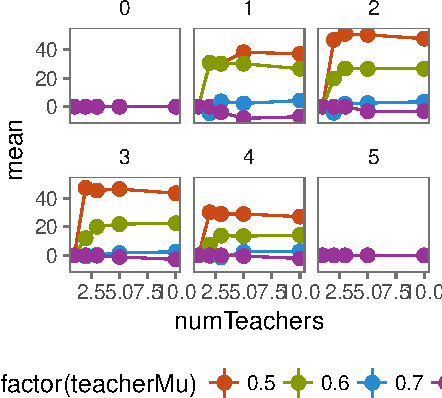
\includegraphics{figs/unnamed-chunk-1-1} \end{CodeChunk}

We hypothesized that for a particular budget constraint and fixed costs
of teachers and assessment, there will be a pareto frontier of possible
allocations of that budget towards teachers and assessments on which
there will be an optimal allocation that maximizes student learning.
Furthermore, we hypoth- esized that the individual results about number
of teachers number of assessments would hold within levels of the other.
This is the unification of all previous simulations into one model that
allows us to introduce a real-world constraint of budget.

In this simulation, we test all integer combinations of number of
teachers between 1 and 10 with number of assessments between 0 and 5. We
assigned the cost of each teacher to be CT = \$10 and the cost of each
assessment CA = \$20.

Our baselines were the worst-performing within-target setup. This always
happened to be the 1-teacher 0-assessment setup, which is consistent
with existing education literature, since a single teacher cannot
significantly differentiate learning, and still has a lot of uncertainty
about student beliefs because no assessments are performed.

Our simulated findings support our hypothesis. There is con- siderable
support for an interaction model between teachers, assessments, and the
target bias, F(7, 112) = 48.61, p\textless{}.001. To visualize the
pareto frontier, we draw a heatmap of scores

above baseline along teacher and assessment axes. We con- tinue to see
that the effects continue to be weaker for more extreme learning
concepts, t(294) = -11.09, p\textless{}.001. This result can be seen in
Figure 5.

Since real-world learning concepts are essentially non- negotiable, the
effectiveness of a particular allocation of bud- get should be judged
within-target, i.e.~an optimal setup within the target bias = 0.8 level
should not be penalized for being ineffective in comparison to the
optimal setup for teaching a target bias of 0.5. We normalized the
information gain above baseline within each target bias level. The
results can be seen in 6

Consistent with Simulation 3, increasing the number of assess- ments on
average improves learning rate up until you cannot afford any more
assessments, across all levels of teachers and target biases. Consistent
with Simulation 2, increasing the number of assessments improves
learning rate up until you cannot afford any more assessments, across
all levels of assessments and target biases of 0.5, 0.6, and 0.7.

An interesting result, however, is that having noisy students diminishes
the effectiveness of increasing the number of teach- ers at certain a
target bias of 0.8. While we aren't sure of the specific mechanism by
which this happens, we suspect that having more teachers introduces
additional risk of wrongly sorting students' prior beliefs, which would
increase the het- erogeneity of classrooms. Since a target belief of 0.8
is a possible target belief to show precisely with 5 examples (the basis
of our simulations) but also extreme enough that most students's prior
belief will fall on one side of that target, in- creasing the number of
teachers might actually reduce the effectiveness of the teacher's choice
of examples. A novel finding that emerged not described in existing
educa- tion literature is that there are different patterns of
optimality along the pareto frontiers. As the extremity of the target
bias moves from 0.5 to 0.7, we see that the IG-optimal allocation of
budget shifts from about 5-6 teachers and 2 assessments towards more
assessments at the expense of the number of teachers.

\section{Discussion}\label{discussion}

Overall, we were able to replicate many real-world findings from
education literature. We found the sorting students into ability level
classrooms, increasing assessment, and decreasing class size all
increase information gain.

One of the more interesting findings was the influence of the target
bias on the effects we were finding. Based on our results, target bias
significantly moderates each of the effects we found. When teaching an
extremely difficult (or easy, given symmetry) learning concept such that
all student prior beliefs are on one side of the concept, the payoffs to
information gain that sorting, class sizes, and assessment have diminish
because regardless of the level of noise, teachers have relative
certainty about the students' relative level of understanding.
Similarly, target biases that are very close to central (around 0.5)
have a lot to gain from diminishing noise in the system.

Finally, we found that the relative effectiveness of number of teachers
and and the number of assessments varies depend- ing on the target
learning concept. We saw that the most optimal distribution of budget on
the pareto frontier shifted towards reducing student noise when the
target bias was more extreme--this seemed consistent with intuition,
since having more teachers doesn't allow them to better select examples
if the administrator produces greater sorting errors, resulting in
heterogeneous classrooms where each teacher has less cer- tainty about
whether their examples will be useful for any particular student or not.

While a lot of aspects of school learning (peer effects, social
dynamics, etc.) are not built into our model and would be difficult to
capture algorithmically, we believe that there is a lot to be gained
from simulating classroom dynamics. Using stochastic modeling is
particularly useful when exploring the effectiveness of education policy
measures for a handful of reasons. Fundamentally, the merits of
stochastic modeling arise from the use of synthetic data. Since the
studies are computer-simulated, there are no human subjects in the stud-
ies, and all of the data is synthetic. This allows researchers to take
greater liberties in experimental design because there are no ethical
concerns. For instance, we can execute a sim- ulation that will
intentionally misclassify synthetic students into classrooms that are
not appropriate for their achievement level to understand the negative
impact doing so has on both the misclassified student and his peers.
Such a study would not be ethically permissible in an actual school.

Furthermore, no two schools are the same, and the use of mod- eling and
synthetic data enables rapid iteration over different simulated schools
with different simulated students. We can quickly test whether the
purported benefit to student learning of various education interventions
holds with, for example, a limited budget, or highly varied student
achievement levels, or immensely large class sizes. There is also no
risk of student subject attrition that may jeopardize real-world school
studies; synthetic students do not exhibit unpredictable absenteeism,
transfer schools, take sick days, etc. As such, we can cus- tomize our
interventions based on school parameters, validate the robustness of our
results, and better infer generalized find- ings about education policy
without incurring astronomical experimental monetary costs nor require
lengthy longitudinal study. With a complete stochastic model, we can
quickly scale the number of hypotheses we test and the variety of
schools we test them on. Our series of simulations are designed to
replicate real-world results from education literature in a
quantitative, simulated fashion. The first few simulations looked at a
lot of existing educational theory in isolation, while our final
simulation attempts to unify these different design aspects of a school
system into a more holistic view. We found that increasing the number of
teachers (and thus decreasing class size) and increasing the amount of
assessment to improve precision about student beliefs increases student
learning, as predicted in real-world school studies.

Importantly, we were able to generate pareto frontiers allo- cating a
fixed shared resource of budget into the dimensions of teachers and
sorting. The ability to make sense of the tradeoffs that school
administrators and policymakers need to make when designing their
schools can help improve educa- tion. This would be particularly
impactful in communities of low socioeconomic status where academic
achievement tends D to be lower because budgets are particularly
constrained and attracting teaching staff is difficult.

Some of the limitations of the present work is in the assump- tions that
we make to build our model. Most obvious is the simplicity of the
learning task we described during the intro- duction. Most real-world
learning tasks are more complicated and may have multiple objectives.
Furthermore learning in the real-world is affected by a lot of more
abstract facets: peer learning and social environment, parenting styles,
stereotype threat, among other things. These are not captured in the
model, and would be difficult to capture in any model. The agnostic
prior beliefs we 1) use for teachers to generate examples from; 2)
generate student prior beliefs from; and 3) create target bias
distributions with are all uniform distri- butions. These are not
necessarily the case. Respectively, 1) teachers may have prior beliefs
about which examples are more effective, akin to pedagogical knowledge
or pedagogical content knowledge (Cochran, 1991); 2) students may tend
towards certain common prior beliefs/misconceptions about a particular
learning concept; 3) more extreme learning concepts may be more rare,
and thus the admin should weight more heavily the pareto frontier of
moderate target bias values.

\section{Acknowledgements}\label{acknowledgements}

This work supported by NSF BCS \#1456077.

\section{References}\label{references}

\setlength{\parindent}{-0.1in} \setlength{\leftskip}{0.125in} \noindent

\hypertarget{refs}{}
\hypertarget{ref-frank2012}{}
Frank, M. C., \& Goodman, N. D. (2012). Predicting pragmatic reasoning
in language games. \emph{Science}, \emph{336}(6084), 998--998.

\end{document}
